\documentclass{report}
\usepackage{float}

% for the image in the title
\usepackage{tikz}

% custom spacing
\usepackage{setspace}
\onehalfspacing

% footer and header
\usepackage{fancyhdr}
% \setlength{\headheight}{15.2pt}

% underlining
\usepackage{ulem}

\usepackage[T1]{fontenc}

% Table of contents link to corresponding sections
\usepackage{hyperref}
\hypersetup{
	colorlinks,
	citecolor=black,
	filecolor=black,
	linkcolor=black,
	urlcolor=black
}

\usepackage{amsmath}
% Remove che "Chapter" string before chapters
\iffalse
\makeatletter
\def\@makechapterhead#1{%
	\vspace*{50\p@}%
	{\parindent \z@ \raggedright \normalfont
		\interlinepenalty\@M
		\Huge\bfseries  \thechapter.\quad #1\par\nobreak
		\vskip 40\p@
}}
\makeatother
\fi

% Fancy chapters
\usepackage[Bjarne]{fncychap}
% options: Sonny, Lenny, Glenn, Conny, Rejne, Bjarne, Bjornstrup

\begin{document}
	
	
	%title page
	\begin{titlepage}
		\begin{figure}[t]
			\centering
\includegraphics[width=0.3\textwidth]{images/unitn-logo}
		\end{figure}
		\begin{center}
			\textsc{ \LARGE{Università degli Studi di Trento \\}}
			\textsc{ \LARGE{Facoltà di Informatica\\ }}
			\textnormal{ \LARGE{Corso di Ingegneria del Software\\}}
			\vspace{30mm}
			\fontsize{10mm}{7mm}\selectfont 
			\textup{Fix Mi \\ Report Finale}\\
		\end{center}
		
		\vspace{25mm}
		
		\centering
		\large Gruppo G43: \\ Giovanni Santini\\ Riginel Ungureanu \\ Valerio Asaro
		
		\vspace{20mm}
		
		\centering{\large{Anno Accademico 2023/2024 \\ Trento }}
		
	\end{titlepage}
	
	
	
	
	% use header and footers
	\pagestyle{fancy}
	\fancyhead[R]{\chaptername\ \thechapter}  % header
	
	%\maketitle
	\tableofcontents
	\newpage
	
	
	
	\section{Scopo del documento}
	
	Il seguente documento contiene una valutazione finale del processo e l'organizzazione per lo sviluppo dell'applicazione "Fix Mi".
	
	\section{Informazioni del Documento}
	
	% table
	\begin{center} % center the table
		\centering
		\begin{tabular}{ |p{4cm}|p{4cm}|  }
			\hline
			\centering Campo & \qquad\qquad Valore \\ % I found no other way...
			\hline
			Titolo del Documento & Report Finale \\
			\hline
			Titolo del Progetto & Fix Mi \\
			\hline
			Autori del Documento &
			Giovanni Santini \\ & Riginel Ungureanu \\ & Valerio Asaro \\
			\hline
			Amministratore Progetto & Riginel Ungureanu\\
			\hline
			Versione del documento & 1.0 \\
			\hline
		\end{tabular}
	\end{center}
	
	
	
\chapter{Report}

\section{Approcci all'ingegneria del software}

\subsection{Blue Tensor}

\subsection{Kanban}

\subsection{IBM}

\subsection{META}

\subsection{U-Hopper}

\subsection{RedHat}

\subsection{Microsoft}

\subsection{Molinari}

\subsection{Marsiglia}

\subsection{APSS \& Trentino.ai}


\section{Organizzazione del lavoro}

Il team di sviluppo ha deciso di adottare una struttura organizzativa orizzontale: una struttura organizzativa in cui tutti i membri della squadra di sviluppo possiedono eque responsabilità.
% Il team ha adottato il seguente organigramma:
Avendo suddiviso il progetto in microservizi è stato possibile gestire la mole di lavoro in maniera asincrona, garantendo una fluidità lavorativa semplice ed efficace: la stesura della documentazione e la scrittura del codice sono state divise in modo equo tra i membri del team di sviluppo
in modo da poter lavorare in contemporanea.
A tale scopo il lavoro è stato diviso in macro obiettivi (rappresentati dai cinque deliverables) a loro volta suddivisi in obiettivi comuni (individuati dai capitoli di ciascun deliverable) e task individuali (rappresentate dalle contribuzioni di ciascun individuo al fine di completare l'obiettivo).
La realizzazione del lavoro è stata suddivisa, specialmente nell'ultimo perido, in più sprints, dove il team di sviluppo si è impegnato a svolgere le proprie task individuali entro una scadenza ben precisa, concordata tra i membri stessi . Durante questi periodi il team si è riunito con frequenza settimanale per discutere riguardo lo stato del progetto, degli obiettivi in corso e quelli successivi.
Per l'organizzazione dello sviluppo il team ha adottato un Workflow basato sul Branching e sulle Pull Requests di GitHub: ogni membro ha lavorato alla propria versione del progetto, inviando le proprie modifiche agli altri membri del gruppo tramite la creazione di "Pull Requests": dopodichè viene effettuato, da parte degli altri membri, un controllo sulla qualità e la correttezza delle modifiche.
Il team di sviluppo ha fatto uso dei seguenti strumenti per lo sviluppo dell'applicazione

\begin{itemize}
	\item Trello
	\begin{itemize}
		\item Software collaborativo per la gestione e l'organizzazione del lavoro di un gruppo.
		\begin{figure}[H]
			\centering
			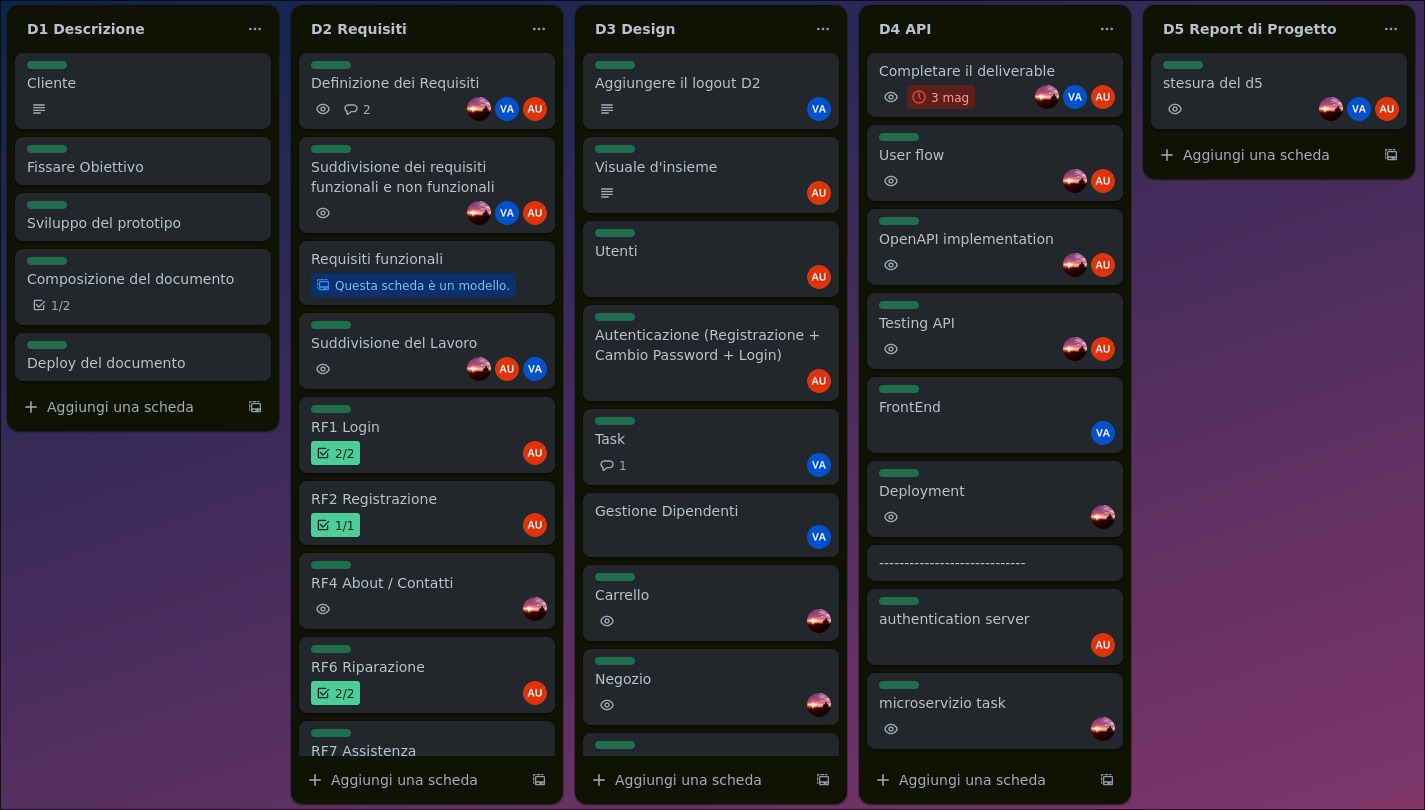
\includegraphics[width=1\textwidth]{images/trello-image.jpg}
			\caption{Organizzazione del lavoro su Trello}
		\end{figure}	
	\end{itemize}
	\item GitHub
	\begin{itemize}
		\item Piattaforma per lo sviluppo di software che permette di creare, immagazzinare, gestire e condividere il codice.
	    \begin{figure}[H]
	    	\centering
	    	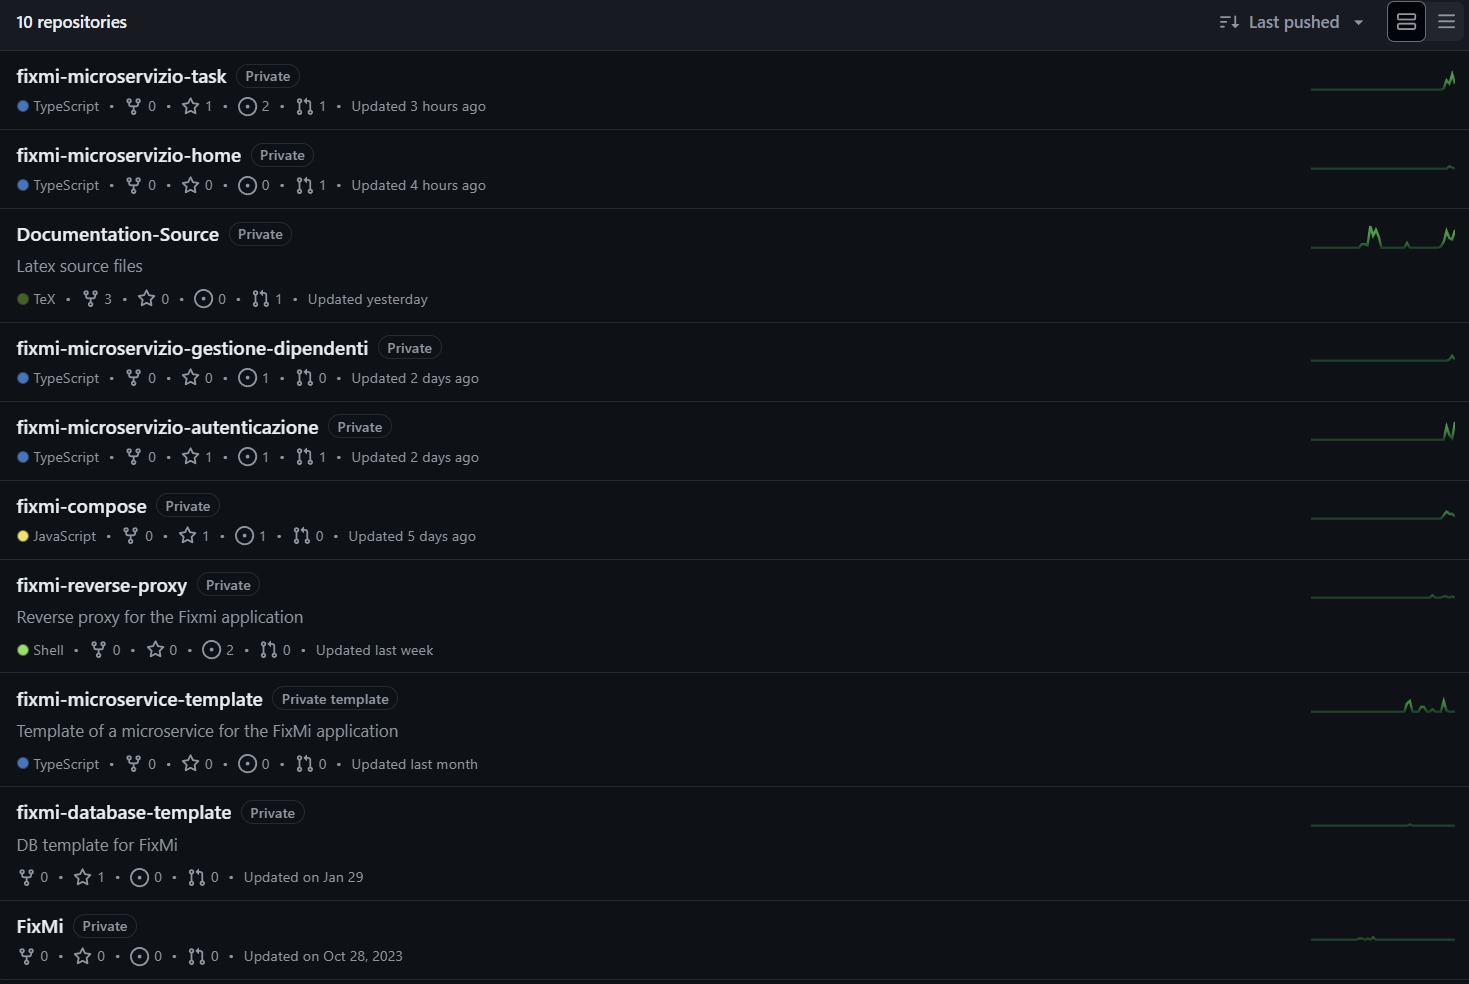
\includegraphics[width=1\textwidth]{images/github-image1.jpg}
	    	\caption{Organizzazione del progetto su GitHub}
	    \end{figure}	
	    \begin{figure}[H]
	    	\centering
	    	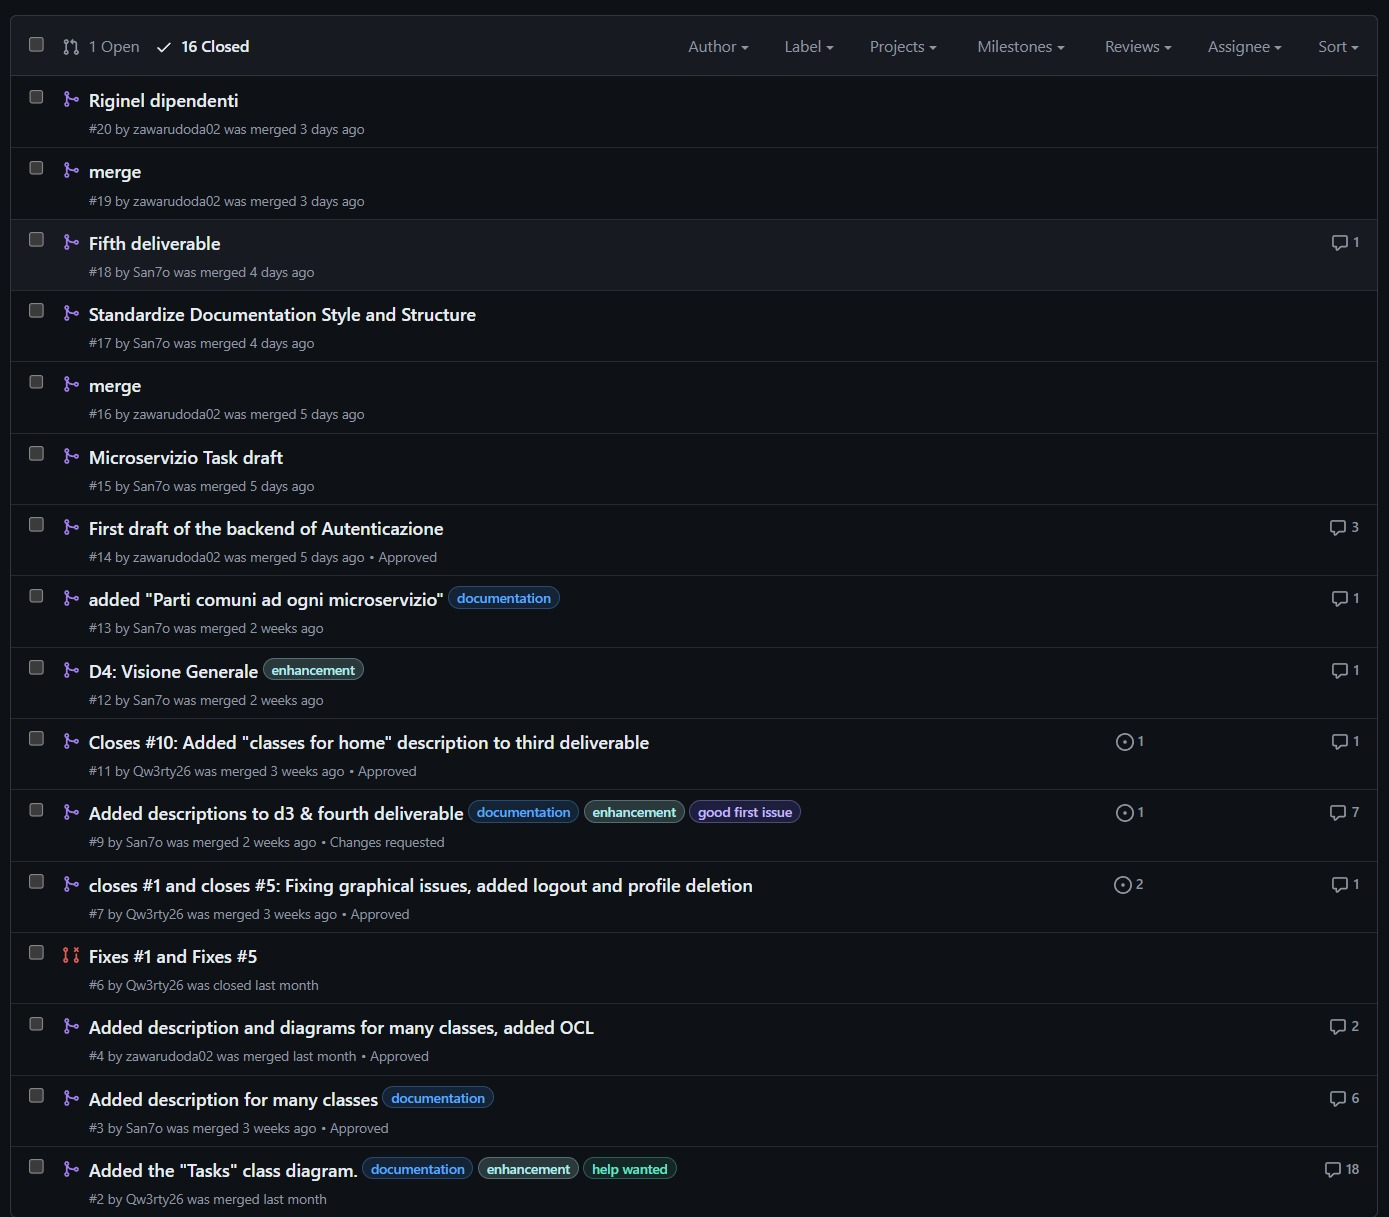
\includegraphics[width=1\textwidth]{images/github-image2.jpg}
	    	\caption{Pull Requests della repository "Documentation Source" su GitHub}
	    \end{figure}	
	\end{itemize}
	\item Google Drive
	\begin{itemize}
		\item Software per la memorizzazione e la sincronizzazione dei files
	\end{itemize}
	\item Draw.io
	\begin{itemize}
		\item Software per la creazione e lo sviluppo di diagrammi
		\begin{figure}[H]
			\centering
			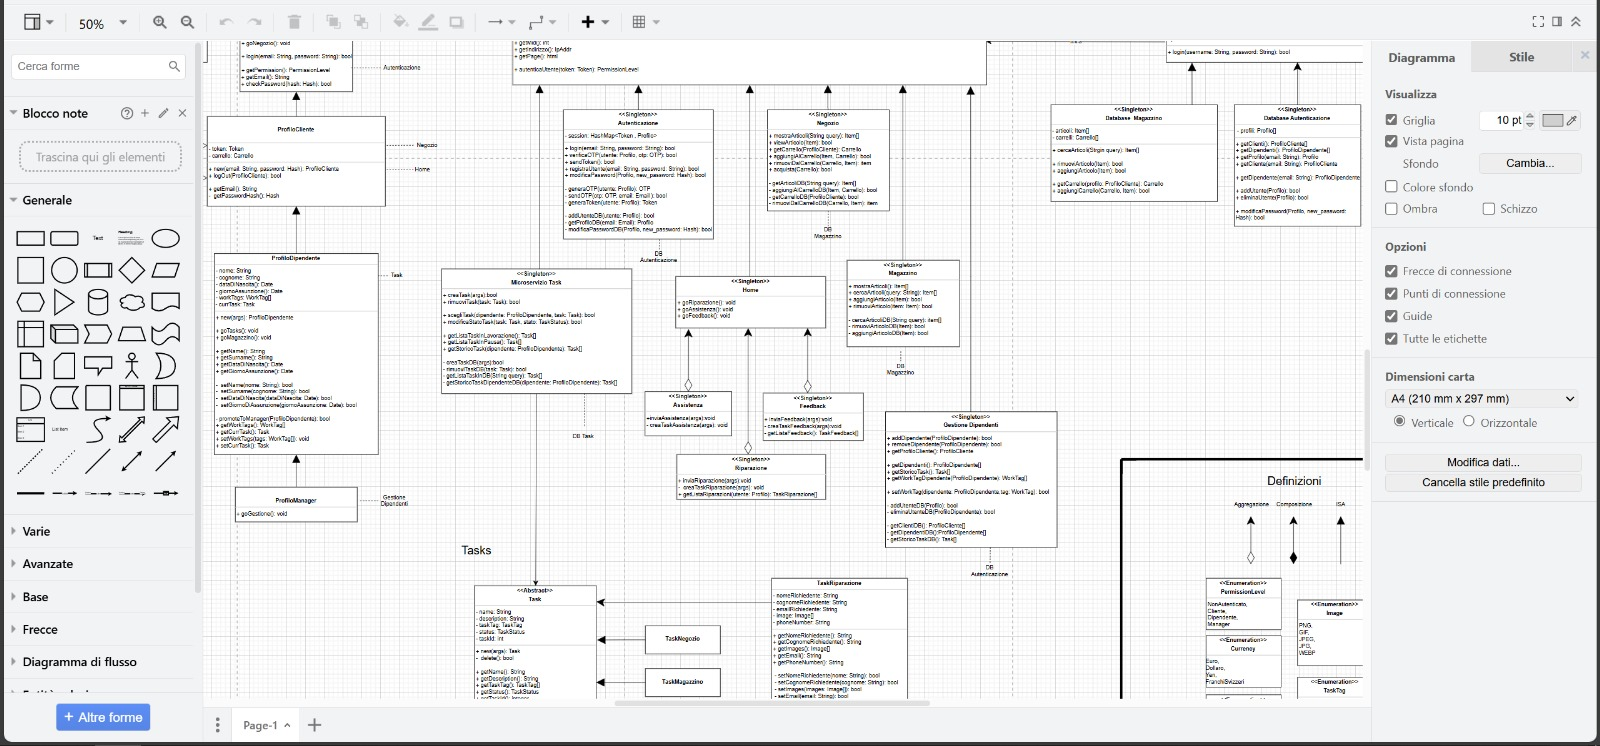
\includegraphics[width=1\textwidth]{images/drawio-image.jpg}
			\caption{Realizzazione del "Diagramma delle Classi" del third-deliverable}
		\end{figure}	
	\end{itemize}
	\item LaTeX
	\begin{itemize}
		\item Un linguaggio MarkUp specializzato nella realizzazione e scrittura di documenti di alta qualità.
		\begin{figure}[H]
			\centering
			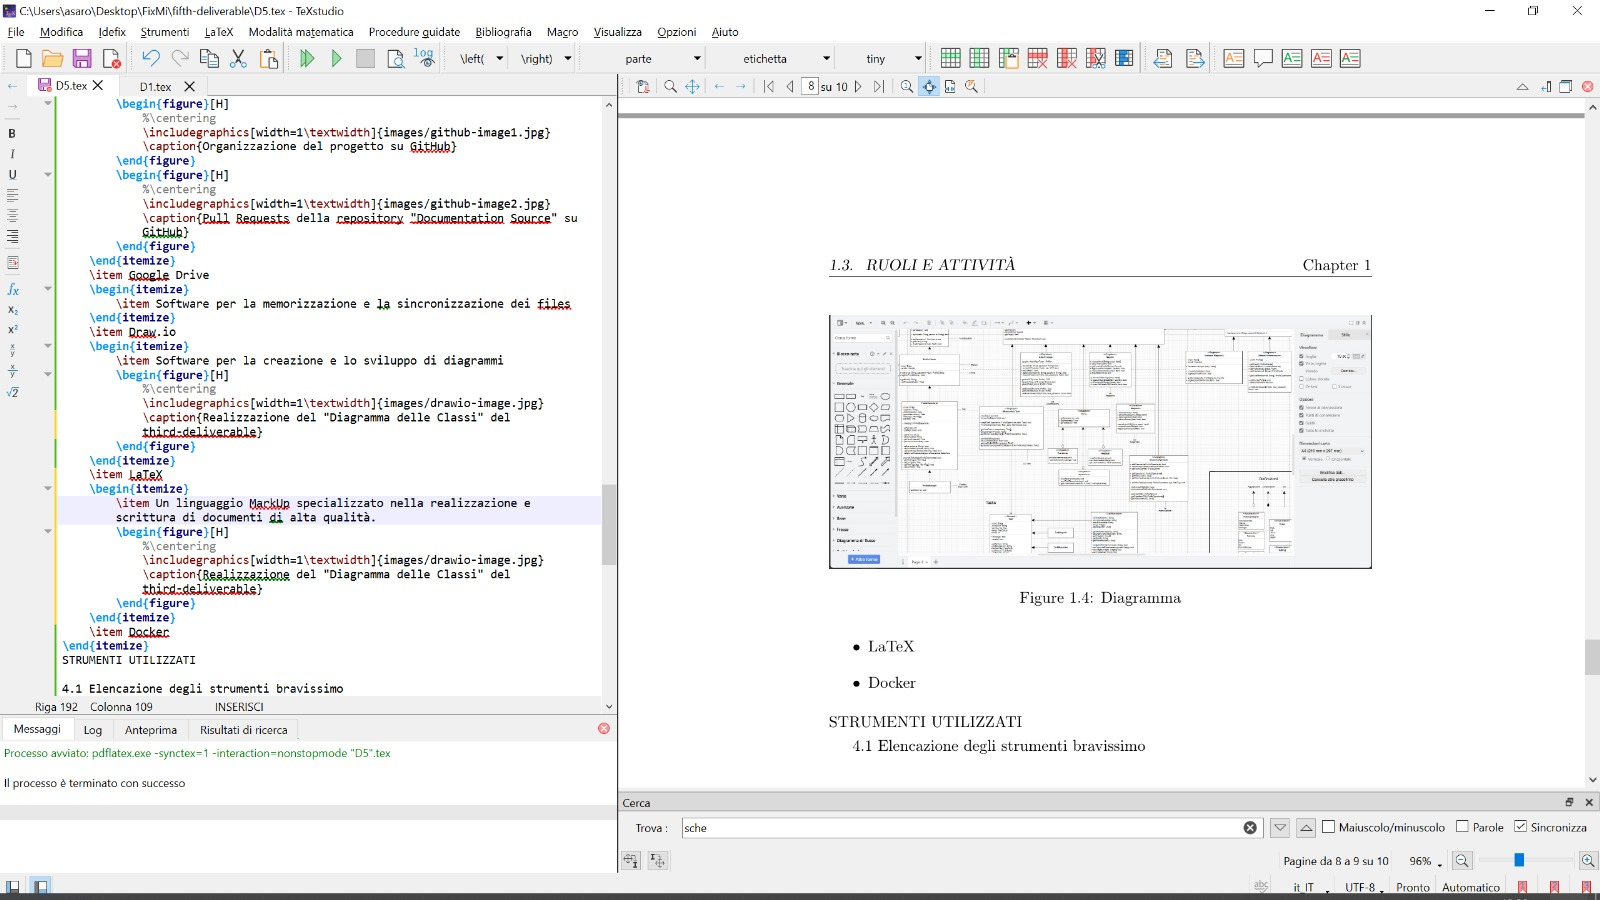
\includegraphics[width=1\textwidth]{images/latex-image.jpg}
			\caption{Scrittura del documento con LaTeX}
		\end{figure}	
	\end{itemize}
	
	\item Docker
	\begin{itemize}
		\item Software per l'esecuzione di processi e programmi in ambiente isolato tramite contenitori minimali e facilmente distribuibili.
		\begin{figure}[H]
			\centering
			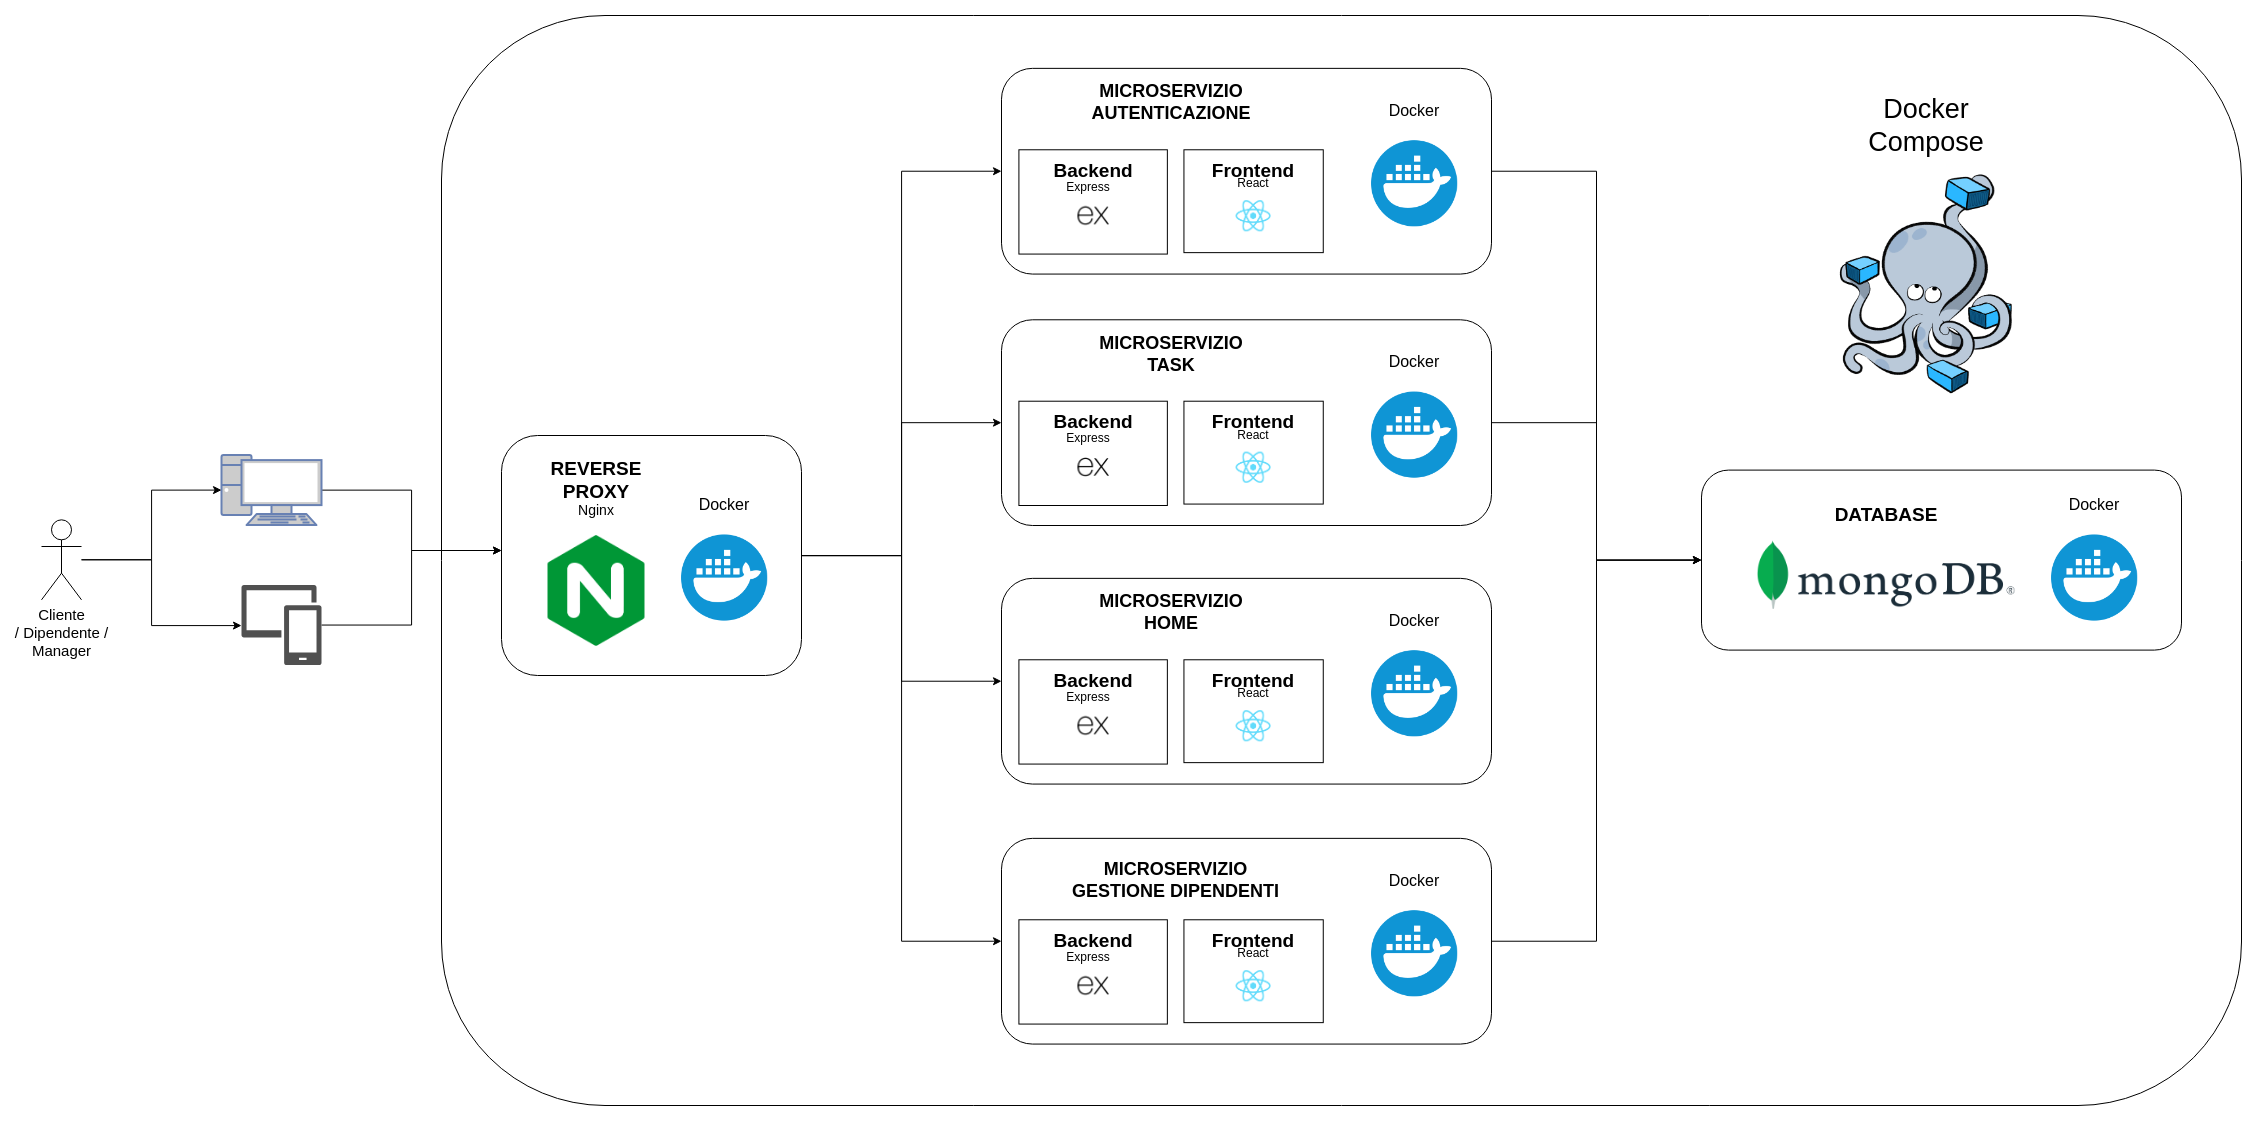
\includegraphics[width=1\textwidth]{images/diagramma_microservizi.png}
			\caption{Struttura del progetto tramite Docker}
		\end{figure}	
	\end{itemize}
	
\end{itemize}



\section{Ruoli e Attività}
% table
\begin{center} % center the table
	\centering
	\begin{tabular}{ |p{4cm}|p{4cm}|p{7cm}|  }
		\hline
		\centering Componente del gruppo & \qquad\qquad Ruolo & \qquad Principali attività \\ % I found no other way...
		\hline
		\centering Giovanni Santini & Sviluppatore BackEnd & Da Compilare \\
		\hline
		\centering Riginel Ungureanu & Responsabile BackEnd e Autenticazione & Da Compilare \\
		\hline
		\centering Valerio Asaro & Responsabile FrontEnd e Designer & 
		 Il compito principale è stato la realizzazione della parte FrontEnd dell'applicazione ma ha anche contribuito alla stesura della documentazione e alla progettazione dell'applicazione.  \\
		\hline
	\end{tabular}
\end{center}

\section{Carico e distribuzione del lavoro}
% table
\begin{center} % center the table
	\centering
	\begin{tabular}{ |p{3cm}|p{1cm}|p{1cm}|p{1cm}|p{1cm}|p{1cm}|p{1cm}|  }
		\hline
		\centering  Membri  &  D1 &  D2 & D3 & D4 & D5 & TOT\\ % I found no other way...
		\hline
		\centering Giovanni Santini & 0 & 0 & 0 & 0 & 0 & 0 \\
		\hline
		\centering Riginel Ungureanu & 0 & 0 & 0 & 0 & 0 & 0 \\
		\hline
		\centering Valerio Asaro & 0 & 0 & 0 & 0 & 0 & 0 \\
		\hline
		\centering TOT & 0 & 0 & 0 & 0 & 0 & 0 \\
		\hline
	\end{tabular}
\end{center}

\section{Criticità}

\section{Autovalutazione}

% table
\begin{center} % center the table
	\centering
	\begin{tabular}{ |p{3cm}|p{1cm}|  }
		\hline
		\centering  Membri  & Voto\\ % I found no other way...
		\hline
		\centering Giovanni Santini & 31 \\
		\hline
		\centering Riginel Ungureanu & 30  \\
		\hline
		\centering Valerio Asaro & 30  \\
		\hline
	\end{tabular}
\end{center}



	
\end{document}